\clearpage\secrel{Managed compilation}\label{manacomp}

\noindent
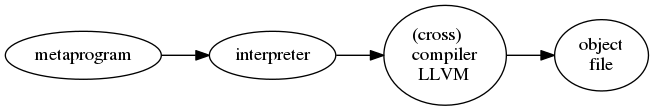
\includegraphics[width=\textwidth]{img/dynacomp.png}

\term{Metacircular managed compiler}

\noindent
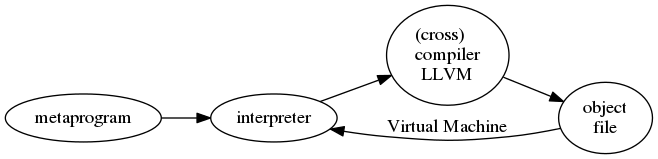
\includegraphics[width=\textwidth]{img/circomp.png}

\noindent
\term{Managed compilation} is \emph{compilation} by a compiler is
\emph{driven by meta\-program}. Classic compilers work in batch mode only: you
put a program for a target system, and get resulting executable code in batch.
Managed compilation extend your abilities to control compilation process in a
very fine grain, much more than macro\note{not available in many languages}.

\bigskip\noindent
\textcolor{red}{The price of power is complexity}: you must write full sized
\term{metaprogram} \emph{builds target code via calls to the compiler
framework}. This complexity can be amortized by using meta-libraries and OOP let
you use helpers and inheritable application templates.

\clearpage\noindent
You can use \term{static managed (cross)compilation} into executable object
files, if you need code for some embedded system, small executable files or
security hardened software system with unmodifiable code.

\bigskip\noindent
But the coolest method for ordinary large computers is running \term{dynamic
compilation} in a runtime, building machine code into RAM (some sort of managed
JIT on steroids). Dynamic compilation allows using \term{flex programming} based
on \emph{self-modifiable programs and nonsequential computation (hyper)graphs}.

